% NSF SaTC 2.0 proposal (NSF 25-515) -- Project Description, RES designation.
% RES: up to $1,200,000 over up to 4 years. Project Description limit: 15 pages.
% Optional add-on: TTE (Transition to Education) -- "SaTC 2.0: RES: TTE: <Title>".
%
% SUBMISSION TARGET DATES (NSF 25-515; these are TARGET dates, not hard deadlines:
%   proposals are accepted anytime, but late ones may miss a review panel):
%   - Last Monday in September, annually (first instance was Sep 29, 2025).
%   - Last Monday in January, annually  (first instance was Jan 26, 2026).
%   Next applicable target dates after June 2026: Mon Sep 28, 2026; Mon Jan 25, 2027.
%   Separate collaborative: NEU (Zhao, lead) + UCCS (Tan) must each submit and link
%   their proposals before the same panel cutoff. Verify against the live solicitation
%   and each institution's internal sponsored-programs deadline before relying on these.
%   Source: https://www.nsf.gov/funding/opportunities/satc-20-security-privacy-trust-cyberspace/nsf25-515/solicitation
% Page budget (15 pages):
%   Introduction/Overview ~2.5
%   Background/Threat model ~2
%   Thrust 1/2/3 ~9
%   Broader Impacts / Timeline / Prior support ~1.5

\documentclass[11pt,oneside,onecolumn,letterpaper]{article}
%\usepackage[OT1]{fontenc}
\usepackage{times}
\usepackage[margin=1in]{geometry}
%\usepackage{amsmath,amssymb,amsfonts}
\usepackage{booktabs}
\usepackage{graphicx}
\usepackage{latexsym}
%\usepackage{subfigure}
\usepackage{wrapfig}
\usepackage{amsthm}
\usepackage{amsmath,amssymb,amsfonts}
\usepackage[hyphens]{url}
\usepackage{pifont}
\usepackage{color}
\usepackage{colortbl}
\usepackage[dvipsnames]{xcolor}
\usepackage[ruled,vlined]{algorithm2e}
\usepackage[square, comma, sort&compress, numbers]{natbib}
\usepackage{pgfgantt}
\usepackage{enumitem}
\usepackage{subcaption}
\usepackage{titlesec}
\usepackage{xspace}
\usepackage{arydshln}
\usepackage{circledsteps}
\usepackage{listings}
\usepackage{stfloats}
\usepackage{comment}
\usepackage{fmtcount}
\usepackage{lipsum}
\usepackage{soul}
\usepackage[textsize=tiny]{todonotes}
\usepackage{multirow}
\usepackage{multicol}
\usepackage{threeparttable}
\usepackage{tcolorbox}
\usepackage{minted}
\usepackage{graphicx}
\usepackage{tikz}
\usetikzlibrary{positioning,arrows.meta,calc,fit}

\newcommand{\rulebox}[1]{
	\begin{tcolorbox}[
		%width=4in,
		boxsep=0pt,
		left=2pt,
		right=2pt,
		top=1pt,
		bottom=1pt,
		boxrule=0.5pt,
		]
		#1
	\end{tcolorbox}
}

\newcommand*\circled[1]{\tikz[baseline=(char.base)]{
		\node[shape=circle,draw,inner sep=0.7pt] (char) {#1};}}

\titlespacing\section{0pt}{4pt plus 2pt minus 2pt}{6pt plus 2pt minus 2pt}
\titlespacing\subsection{0pt}{4pt plus 2pt minus 2pt}{2pt plus 2pt minus 2pt}
\titlespacing\subsubsection{0pt}{4pt plus 4pt minus 2pt}{2pt plus 2pt minus 2pt}

\titleformat{\section}
{\fontsize{12}{15}\bfseries}{\thesection}{1em}{}

\titleformat{\subsection}
{\fontsize{11}{15}\bfseries}{\thesubsection}{1em}{}

% Inline review/comment macro (highlighted). Wrap notes you do NOT want in the final PDF.
\newcommand{\ziming}[1]{%
  \begingroup
  \definecolor{hlcolor}{RGB}{20, 255, 20}\sethlcolor{hlcolor}%
  \textcolor{black}{\hl{\textit{\textbf{Ziming:} #1}}}%
  \endgroup
}

% Salient placeholder/TODO marker -- bright red bold so unfilled gaps are impossible to miss
% in the compiled PDF. Robust in captions, long text, and special characters. Remove before submission.
\definecolor{todored}{rgb}{0.85,0,0}
\newcommand{\TODO}[1]{\textcolor{todored}{\textbf{[TODO: #1]}}}

% Placeholder for a not-yet-available photo/figure: a red-framed gray box with a label.
% Usage: \photoplaceholder[width]{description}. Box height is \phheight (default 2.6cm);
% set \phheight locally (e.g. inside a subfigure, where it auto-resets) to match a photo.
\newlength{\phheight}\setlength{\phheight}{2.6cm}
\newcommand{\photoplaceholder}[2][0.3\textwidth]{%
  \fcolorbox{red}{gray!12}{\parbox[b][\phheight][c]{#1}{\centering\footnotesize\textcolor{red}{\textbf{[PHOTO: #2]}}}}%
}

% ---------------------------------------------------------------------------
% TODO(glitching): name the system(s) / artifacts this proposal introduces.
% These are placeholders carried over from the template -- rename or remove.
% ---------------------------------------------------------------------------
\newcommand{\sysname}{{\scshape Forge}\xspace}
\newcommand{\ctfplatform}{\textsc{PwnIoT.Academy}\xspace}

% Thrust titles. Arc: understand (T1) -> detect (T2) -> defend (T3), unified by the compiler.
% Refine wording as the proposal matures.
\newcommand{\thrustone}{Characterizing the Compiler-Enlarged Glitching Attack Surface}
\newcommand{\researchoneone}{Task 1.1: Attributing Fault-Injection Surface to Compiler Transformations}
\newcommand{\researchonetwo}{Task 1.2: A Metric to Quantify the Glitching Attack Surface of Compiled Code}

\newcommand{\thrusttwo}{Automated Discovery of Compiler-Induced Glitching Vulnerabilities}
\newcommand{\researchtwoone}{Task 2.1: A Fault Model and Vulnerability Analysis Framework}
\newcommand{\researchtwotwo}{Task 2.2: Automated, Scalable Glitching Bug Finding}
\newcommand{\researchtwothree}{Task 2.3: Exploitability Triage and Validation}

\newcommand{\thrustthree}{Automated, Cost-Aware Compiler Hardening with Fault-Resistance Guarantees}
\newcommand{\researchthreeone}{Task 3.1: Selective, Cost-Optimal Countermeasure Placement}
\newcommand{\researchthreetwo}{Task 3.2: Fault-Aware Code Generation to Avoid Introducing Surface}
\newcommand{\researchthreethree}{Task 3.3: Verifying Residual Security Under a Bounded Fault Model}

\newcommand{\cmark}{\ding{51}}%
\newcommand{\xmark}{\ding{55}}%

\definecolor{codegreen}{rgb}{0,0.6,0}
\definecolor{codegray}{rgb}{0.5,0.5,0.5}
\definecolor{codepurple}{rgb}{0.58,0,0.82}
\definecolor{backcolour}{rgb}{0.95,0.95,0.92}

\pgfkeys{/csteps/inner xsep=1.5pt}
\pgfkeys{/csteps/inner ysep=1.5pt}

\colorlet{punct}{red!60!black}
\definecolor{background}{HTML}{EEEEEE}
\definecolor{delim}{RGB}{20,105,176}
\colorlet{numb}{magenta!60!black}

\lstdefinestyle{mystyle}{
    backgroundcolor=\color{backcolour},
    commentstyle=\color{codegreen},
    keywordstyle=\color{magenta},
    numberstyle=\tiny\color{codegray},
    stringstyle=\color{codepurple},
    basicstyle=\ttfamily\tiny,
    breakatwhitespace=false,
    breaklines=true,
    captionpos=b,
    keepspaces=true,
    numbers=none,
    numbersep=5pt,
    showspaces=false,
    showstringspaces=false,
    showtabs=false,
    tabsize=2,
    literate=
     *{0}{{{\color{numb}0}}}{1}
      {1}{{{\color{numb}1}}}{1}
      {2}{{{\color{numb}2}}}{1}
      {3}{{{\color{numb}3}}}{1}
      {4}{{{\color{numb}4}}}{1}
      {5}{{{\color{numb}5}}}{1}
      {6}{{{\color{numb}6}}}{1}
      {7}{{{\color{numb}7}}}{1}
      {8}{{{\color{numb}8}}}{1}
      {9}{{{\color{numb}9}}}{1}
      {:}{{{\color{punct}{:}}}}{1}
      {,}{{{\color{punct}{,}}}}{1}
      {\{}{{{\color{delim}{\{}}}}{1}
      {\}}{{{\color{delim}{\}}}}}{1}
      {[}{{{\color{delim}{[}}}}{1}
      {]}{{{\color{delim}{]}}}}{1}
}

\newcounter{goal}
\newcommand{\goal}[1]{
  \stepcounter{goal}
  \textbf{G\padzeroes[1]\decimal{goal}. #1}
}

\lstset{style=mystyle}

\lstdefinestyle{armasm}{
  basicstyle=\scriptsize\ttfamily,
  frame=single,
  framesep=2pt,
  numbers=none,
  tabsize=2,
  columns=fullflexible,
  literate={},
  keywords={cmp,bgt,beq,bne,bl,b,movs,mov,adds,uxtb,cbnz,cbz,ldrb,strb,pop,push,ldr},
  keywordstyle={\bfseries\color{blue!60!black}},
  commentstyle={\itshape\color{gray!50!black}},
  morecomment=[l]{;},
  escapeinside={|}{|},
}
\newcommand{\glitchhl}[1]{{\setlength{\fboxsep}{0pt}\colorbox{yellow!50}{\strut\scriptsize\ttfamily#1}}}

\graphicspath{{./figs/}}

\begin{document}

\pagenumbering{gobble}

\begin{center}
{\large{\bf
% Separate collaborative submission (NEU lead Zhao + UCCS lead Tan). Both linked proposals carry
% the identical title with the "Collaborative Research:" prefix (NSF 25-515, RES designation).
Collaborative Research: SaTC 2.0: RES: \sysname: Characterizing, Finding, and Reducing Compiler-Introduced Glitching Vulnerabilities in Embedded Systems}}
\end{center}

% !TEX root = ProjectDescription.tex
\section{Overview and Objectives}

Embedded systems are ubiquitous computing devices deployed across critical infrastructure, consumer electronics, medical devices, industrial control systems, and IoT applications.
These systems range from microcontroller units (MCUs) that power sensors and edge devices to more capable embedded processors in automotive systems, smart home devices, and industrial controllers.
They are essential to everyday life, with billions of embedded devices deployed globally and projected to grow to trillions by 2035~\cite{Philip2021route}.
While the benefits of these systems are unparalleled, unfortunately, they are susceptible to cyberattacks that are occurring at unprecedented levels, and which often have severe consequences ranging from loss of life~\cite{FDA2019} to homeland security breaches~\cite{stellios2018survey}.
To ensure our embedded and IoT infrastructure is built on a trustworthy and secure foundation, the ``IoT Cybersecurity Improvement Act of 2019" (S.734 in the Senate)~\cite{s734} highlights the need for urgent actions on embedded systems security.

In response to these persistent software vulnerabilities, the cybersecurity community and government agencies have pursued multiple complementary strategies to mitigate memory corruption attacks on embedded systems.
One major effort pursues defensive techniques that continue to use C and C++ while deploying compiler-based and runtime mitigations—including stack canaries, address space layout randomization (ASLR), data execution prevention (DEP), control-flow integrity (CFI), and software fault isolation (SFI)—to reduce the exploitability of memory corruption bugs without requiring language rewrites.
A parallel and increasingly strategic effort involves transitioning to memory-safe programming languages: the White House and federal agencies have invested significant effort in promoting memory-safe languages as a defense against memory corruption vulnerabilities~\cite{whitehouse2024memory}, with major initiatives including DARPA's memory-safety focused research programs~\cite{darpa2024ssith} underscoring the importance of moving embedded system development away from unsafe languages like C and toward memory-safe alternatives such as Rust.
Both approaches have made measurable progress: as we showed in our CCS 2025 paper analyzing MITRE's Embedded Capture-The-Flag (eCTF) competitions~\cite{ma2025ectf}, both the deployment of defensive techniques in C/C++ and the adoption of Rust are increasing, with memory-corruption-based vulnerabilities declining significantly across competition rounds.

Yet both memory-safe languages and hardened C/C++ share a fundamental limitation: they only protect the software layer.
Embedded systems operate under constraints that expose them to a different class of attacks altogether: they need hardware access, run on tight resource budgets, and execute on processors with minimal built-in security.
When software defenses mature, attackers simply shift their approach—they move to hardware-level attacks that exist below the software layer entirely.
In recent eCTF competitions (as documented in our CCS 2025 analysis~\cite{ma2025ectf}), we're seeing exactly this play out: multiple teams are successfully using fault injection to compromise embedded systems, whether those systems are running hardened C/C++ code or Rust.
This means neither approach solves the problem—fault injection is orthogonal to memory safety, and it's a threat that remains largely unaddressed in embedded systems security research.

\subsection{Proposed Research}

\begin{figure}[t]
\centering
\resizebox{\textwidth}{!}{%
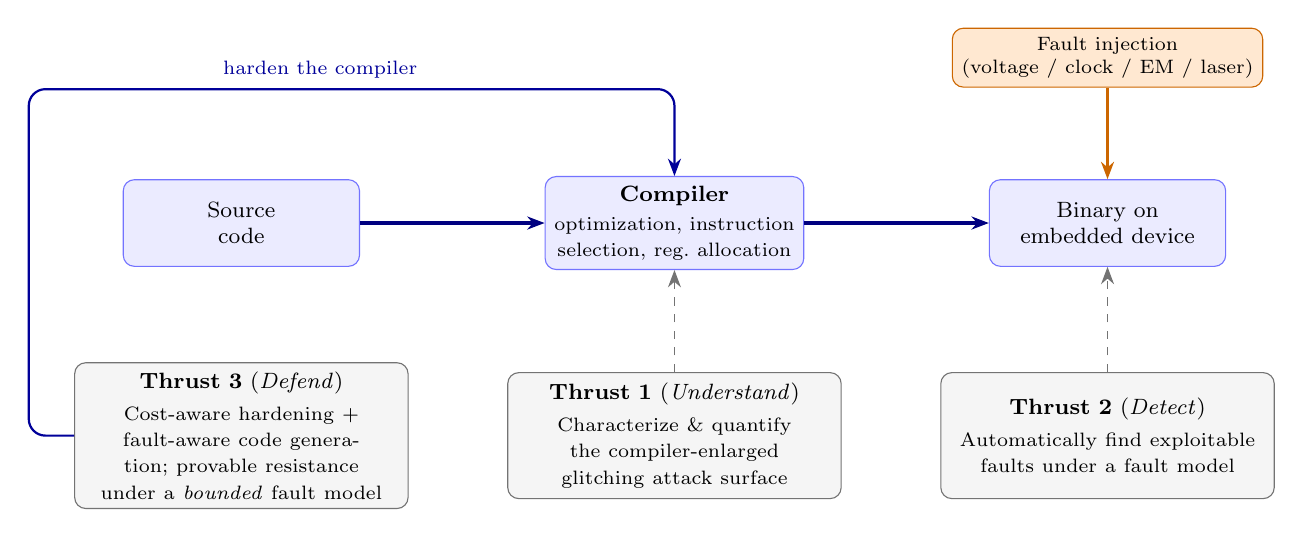
\begin{tikzpicture}[
  font=\footnotesize,
  >={Stealth[length=2.2mm]},
  layer/.style={draw=blue!55, fill=blue!8, rounded corners, align=center, minimum width=3cm, minimum height=1.1cm},
  glitchbox/.style={draw=orange!80!black, fill=orange!18, rounded corners, align=center, font=\scriptsize},
  thrust/.style={draw=black!55, fill=black!4, rounded corners, align=center, minimum height=1.6cm},
  pipe/.style={->, very thick, blue!50!black},
  ann/.style={->, dashed, black!55},
]
% --- implementation layers (pipeline), spread across the full column ---
\node[layer] (src)  at (2,0)    {Source\\code};
\node[layer] (comp) at (7.5,0)  {\textbf{Compiler}\\[1pt]{\scriptsize optimization, instruction}\\{\scriptsize selection, reg.\ allocation}};
\node[layer] (bin)  at (13,0)   {Binary on\\embedded device};
\draw[pipe] (src)  -- (comp);
\draw[pipe] (comp) -- (bin);
% --- to-be-addressed issue: fault injection ---
\node[glitchbox] (glitch) at (13,2.1) {Fault injection\\(voltage / clock / EM / laser)};
\draw[->, very thick, orange!80!black] (glitch) -- (bin);
% --- thrusts in one row ---
\node[thrust, text width=4.0cm] (t3) at (2,-2.7)   {\textbf{Thrust 3} (\mbox{\emph{Defend}})\\[2pt]{\scriptsize Cost-aware hardening + fault-aware code generation; provable resistance under a \emph{bounded} fault model}};
\node[thrust, text width=4.0cm] (t1) at (7.5,-2.7) {\textbf{Thrust 1} (\mbox{\emph{Understand}})\\[2pt]{\scriptsize Characterize \& quantify the compiler-enlarged glitching attack surface}};
\node[thrust, text width=4.0cm] (t2) at (13,-2.7)  {\textbf{Thrust 2} (\mbox{\emph{Detect}})\\[2pt]{\scriptsize Automatically find exploitable faults under a fault model}};
\draw[ann] (t1.north) -- (comp.south);
\draw[ann] (t2.north) -- (bin.south);
% --- Thrust 3 feedback loop into the compiler ---
\draw[->, thick, blue!60!black, rounded corners=6pt]
  (t3.west) -- (-0.7,-2.7) -- (-0.7,1.7) -- (7.5,1.7) -- (comp.north);
\node[blue!60!black, font=\scriptsize] at (3.0,1.95) {harden the compiler};
\end{tikzpicture}%
}
\caption{Overview of \sysname. The three-thrust agenda follows an \emph{understand $\rightarrow$ detect $\rightarrow$ defend} arc unified by the compiler. To-be-addressed issues are shown in {\color{orange!85!black}orange} and implementation layers in {\color{blue!60!black}blue}: the compiler enlarges the glitching attack surface (Thrust~1), which we discover automatically (Thrust~2) and then reduce by feeding cost-aware, verifiable hardening back into the compiler (Thrust~3).}
\label{fig:overview}
\end{figure}

As shown in Figure~\ref{fig:overview}, this proposal pursues a three-thrust agenda, \sysname, that follows an \emph{understand $\rightarrow$ detect $\rightarrow$ defend} arc unified by the compiler.
% TODO(glitching): state the overarching scientific goal in 1-2 bold sentences (cf. previous proposal), then the per-thrust paragraphs below.

\noindent\textbf{Thrust 1: \thrustone.}
% Compilers (optimization passes, instruction selection, register allocation) can introduce
% single points of failure and enlarge the fault-injection surface. Characterize and attribute this.

\noindent\textbf{Thrust 2: \thrusttwo.}
% A fully automated system to discover glitching vulnerabilities under a fault model.
% Framed as defensive bug-finding.

\noindent\textbf{Thrust 3: \thrustthree.}
% Close the loop: re-engineer the compiler to reduce the surface selectively (minimal overhead)
% and prove residual resistance under a bounded fault model. (We reduce, not eliminate -- a
% determined attacker with enough attempts can always inject some fault.)

\noindent\textbf{Novelty and relation to prior work.}
\textbf{Our key observation is that the compiler shapes a system's exposure to \emph{physical} fault injection in the same way it is known to shape its exposure to \emph{software} security bugs, yet only the software side has been studied.}
A closely related line of prior research shows that compilers can introduce software security weaknesses: optimizations delete memory-scrubbing operations~\cite{yang2017deadstore}, exploit undefined behavior to remove safety and security checks~\cite{wang2013undefined}, and more broadly open a ``correctness-security gap'' in which a transformation that preserves functional correctness nonetheless violates a security property~\cite{dsilva2015correctness}; a recent systematic study finds these compiler-introduced security bugs widespread across modern toolchains and optimization passes~\cite{xu2023silent}.
Our own work in the MITRE embedded CTF competition makes the pattern concrete: compiler optimizations silently removed \texttt{memset} calls intended to scrub AES keys from the stack, leaving sensitive data recoverable after it was meant to be erased~\cite{ma2025ectf}.
\sysname carries the same observation to physical fault injection: to our knowledge, no prior work characterizes, detects, or reduces the glitching attack surface that the compiler introduces, and \sysname is the first to treat the compiler as both the cause and the remedy of this physical-layer exposure.

\subsection{Relevance to SaTC}

This proposal directly serves the mission of the NSF SaTC~2.0 program (NSF~25-515), which ``aims to build trust in global cyber ecosystems'': ecosystems that, as the solicitation observes, have grown to involve ``hardware, software, networks, data, people, organizations, countries, and the physical world.''
\sysname addresses the seam between software and the physical world: fault-injection (glitching) attacks that violate the assumptions software, and the compilers that produce it, make about correct execution.
The effort falls squarely within the program's \emph{Computing and Communication Systems} scope, spanning hardware security, embedded systems, and trusted execution, and it also contributes to \emph{Foundations} through the formal, bounded-fault-model resistance guarantees developed in Thrust~3.
By characterizing (Thrust~1), automatically discovering (Thrust~2), and reducing (Thrust~3) compiler-introduced glitching vulnerabilities, \sysname strengthens the trustworthiness of the embedded and IoT devices that underpin transportation, healthcare, energy, and other critical infrastructure, advancing SaTC's goal of a resilient cyber ecosystem.
% TODO(glitching): if pursuing the optional TTE (Transition to Education) designation, add 1-2 sentences here on the integrated education plan.

\subsection{PI Qualifications}

The two PIs bring complementary expertise across the compiler and the hardware/software boundary that \sysname targets, on top of a broad record in systems and software security~\cite{zhang2019icore, zhao2011automatic, zhao2013using, tang2017nivanalyzer, jing2014morpheus, jing2014riskmon, jing2015towards, li2022understanding}.

\noindent\textbf{PI Zhao (Lead PI, Northeastern University)} is an Associate Professor at the Khoury College of Computer Sciences who has focused extensively on embedded system security and on the microarchitectural hardware/software boundary, the same layer at which glitching operates.
He designed CacheLight~\cite{gutierrez2018cachelight} and SmokeBomb~\cite{cho2020smokebomb} to mitigate cache side-channel attacks on the ARM architecture, and uncovered the Prime+Count cross-world covert channel on ARM TrustZone~\cite{cho2018prime}.
His group has crawled thousands of real-world embedded firmware samples to identify and analyze their vulnerabilities~\cite{nino24firware}, built trusted execution environments for embedded and IoT systems~\cite{zhao24tee, byotee24}, designed low-overhead control-flow attestation for microcontroller-based systems~\cite{armanuzzaman2025enola}, and works directly with electromagnetic emanations from embedded devices~\cite{Moradihaghighi2026fuzzemup}, the same physical channel exploited by EM fault injection.
Like fault injection, these attacks exploit physical and microarchitectural behavior rather than software bugs, giving PI Zhao direct experience with the threat model, measurement, and defenses this proposal targets.
His research has garnered several awards, including the \textbf{SACMAT Test-of-Time Award 2024} and \textbf{distinguished paper awards} at \textbf{USENIX Security 2019}, \textbf{AsiaCCS 2022}, and \textbf{CODASPY 2014}.
% TODO(glitching): verify award attribution now that the team changed -- the prior proposal listed these as team awards shared with Co-PI Kirda; NDSS 2011 (Kirda's EXPOSURE) has been removed.
He co-founded the USENIX Symposium on Vehicle Security and Privacy (VehicleSec) as modern vehicles are full of embedded systems, and has a track record of open-sourcing prototypes~\cite{ma2023dac, zhang2018secore, cho2020smokebomb, fengformal2021, lamp2019exsol} and transitioning them to patents and products~\cite{cho2020smokebomb, ahn2015methods, tu2017systems, isign}, e.g., in Samsung Tizen OS~\cite{Tizen}.

\noindent\textbf{PI Tan (University of Colorado Colorado Springs)} is an Assistant Professor who specializes in the security of embedded and ARM Cortex-M systems, with a focus on control-flow security and the architectural limits of deploying modern defenses on microcontroller-based systems.
Her work in this area includes a comprehensive bottom-up study of Arm Cortex-M security~\cite{tan24sok}, an analysis of the effectiveness of stack canaries on microcontroller systems~\cite{tan24canary}, and SHERLOC, a secure and holistic control-flow violation detector for embedded systems~\cite{tan2023sherloc}.
PI Tan will lead the hardware glitching testbed and on-device validation effort (Thrust~2). % TODO(glitching): confirm title/dept; add fault-injection-specific works if available.

\noindent\textbf{Joint efforts.}
The PIs have a sustained record of working together on embedded control-flow security, including attack-and-defense studies of return-to-non-secure and cross-state control-flow hijacking on Cortex-M TrustZone~\cite{ma2023dac, ma2025microft} and debugger-based asynchronous control-flow integrity for embedded systems~\cite{wang24insect}, giving them shared familiarity with the compiler and hardware/software boundary that glitching subverts.
Most relevant to \sysname, the PIs have jointly led teams in the MITRE Embedded Capture-the-Flag (eCTF) competition for six consecutive years and have published studies distilling its security lessons~\cite{ma2025ectf, ma2026wejust}, placing among the top teams \TODO{confirm years/placements}.
In these competitions, the team used power/voltage glitching and related fault-injection techniques to bypass secure boot, defeat firmware protections, and extract secrets from the embedded targets \TODO{add concrete examples}, giving the PIs an attacker's-eye view of the threats \sysname sets out to characterize, find, and reduce.


% !TEX root = ProjectDescription.tex
% Placeholder kept in the input chain (matches the funded-proposal structure).
% Use this for any results-from-prior content that should appear right after the intro,
% or leave empty -- "Results from Prior NSF Support" is rendered near the end of ProjectDescription.tex.


\section{Background}

% TODO(glitching): Provide the technical background a reviewer needs.
%  - Fault injection mechanisms: voltage/clock glitching, EMFI, laser FI, Rowhammer-adjacent.
%  - Fault models (instruction skip, bit flip, data corruption) and how faults map to exploits.
%  - Relevant hardware/SoC features and existing countermeasures.

\section{System and Threat Models}

% TODO(glitching): Define the system model (target platform, assets) and the
% threat model (attacker capabilities, physical access assumptions, trust boundaries).


\section{Research Thrusts}

% This \section header introduces all thrusts; thrusts 2 and 3 continue with \subsection.

\subsection{Thrust 1: \thrustone}
\label{sec:thrust1}

\noindent\textbf{Problem Statement.}
% TODO(glitching): 2-4 sentences. What is the gap?
%   - Fault-injection defenses are reasoned about at the source/ISA level, but the binary that
%     actually runs is produced by the compiler.
%   - Optimization, instruction selection, register allocation, and scheduling can collapse
%     redundant checks, create single points of failure, and otherwise enlarge the surface a
%     glitch can exploit -- invisibly to the developer.
%   - This compiler-introduced surface is neither characterized nor quantified today.

\smallskip
\noindent\textbf{Research Questions.}
\begin{itemize}[leftmargin=*,nosep]
  \item \textbf{RQ1.1:} Which compiler transformations (optimization passes, instruction selection, register allocation, scheduling) introduce or enlarge the glitching attack surface, and by how much?
  \item \textbf{RQ1.2:} How can the glitching attack surface of compiled code be \emph{quantified} so it can be compared across compilers, optimization levels, and target ISAs?
  \item \textbf{RQ1.3:} Do some compiler decisions \emph{reduce} the surface, revealing low-cost levers for Thrust~3?
\end{itemize}

\smallskip
\noindent\textbf{Approach Overview.}
% TODO(glitching): one paragraph tying the tasks below to the RQs above.

\subsubsection{\researchoneone}
\noindent\textbf{Goal.} % TODO(glitching)
\noindent\textbf{Approach.} % TODO(glitching): differential analysis across passes / -O levels; map source-level checks to emitted instructions.
\noindent\textbf{Expected Outcome.} % TODO(glitching)

\subsubsection{\researchonetwo}
\noindent\textbf{Goal.} % TODO(glitching)
\noindent\textbf{Approach.} % TODO(glitching): define a surface metric (e.g., exploitable single-fault sites per function) and a measurement methodology.
\noindent\textbf{Expected Outcome.} % TODO(glitching)


% !TEX root = ProjectDescription.tex
\subsection{Thrust 2: \thrusttwo}
\label{sec:thrust2}

\noindent\textbf{Problem Statement.}
% TODO(glitching): 2-4 sentences. Frame defensively (bug-finding), not as attack tooling.
%   - Finding glitching vulnerabilities today is largely manual, target-specific, and slow.
%   - Thrust 1 shows the compiler-introduced surface is large; we need to find the exploitable
%     subset automatically, at scale, before adversaries do.
%   - Challenge: a faithful-yet-tractable fault model, and search that scales to real binaries.

\smallskip
\noindent\textbf{Research Questions.}
\begin{itemize}[leftmargin=*,nosep]
  \item \textbf{RQ2.1:} What fault model(s) faithfully capture real glitching effects (instruction skip, bit flip, data corruption) on compiled embedded code while remaining tractable for automated analysis?
  \item \textbf{RQ2.2:} How can exploitable fault-injection vulnerabilities be discovered \emph{automatically and scalably} in compiled binaries?
  \item \textbf{RQ2.3:} How do we triage and \emph{validate} candidates to separate genuinely exploitable faults from benign ones, ideally confirming on real hardware?
\end{itemize}

\smallskip
\noindent\textbf{Approach Overview.}
% TODO(glitching): one paragraph tying the tasks below to the RQs above.

\subsubsection{\researchtwoone}
Formalizes a tractable fault model capturing real glitching effects (instruction skip, bit flip, data corruption) and defines a binary-level vulnerability condition for automated analysis.
\noindent\textbf{Goal.} % TODO(glitching)
\noindent\textbf{Approach.} % TODO(glitching): formalize fault model(s) and a binary-level vulnerability condition.
\noindent\textbf{Expected Outcome.} % TODO(glitching)

\subsubsection{\researchtwotwo}
Builds an automated search engine combining fault simulation, symbolic execution, and/or fuzzing under the Task~2.1 fault model to discover exploitable sites in compiled binaries at scale.
\noindent\textbf{Goal.} % TODO(glitching)
\noindent\textbf{Approach.} % TODO(glitching): automated search -- fault simulation / symbolic execution / fuzzing under the fault model.
\noindent\textbf{Expected Outcome.} % TODO(glitching)

\subsubsection{\researchtwothree}
Ranks candidate vulnerabilities by exploitability and confirms high-priority findings on a physical hardware glitching testbed, establishing ground truth for Thrusts~1 and~3.
\noindent\textbf{Goal.} % TODO(glitching)
\noindent\textbf{Approach.} % TODO(glitching): exploitability triage; validation on a hardware glitching testbed.
\noindent\textbf{Expected Outcome.} % TODO(glitching)


% !TEX root = ProjectDescription.tex
\subsection{Thrust 3: \thrustthree}
\label{sec:thrust3}

\noindent\textbf{Problem Statement.}
% TODO(glitching): 2-4 sentences.
%   - Existing fault-injection countermeasures are applied blanket (2-3x overhead) or by hand.
%   - Since the compiler creates the surface (Thrust 1) and we can locate the exploitable subset
%     (Thrust 2), the compiler can also shrink it -- selectively, at minimal cost, with guarantees.
%   - We reduce, not eliminate: full elimination is impossible under physical fault injection.
%     The defensible claim is provable resistance to a BOUNDED number of faults (fault model).
%   - Challenge: cost-optimal placement + a defensible claim of residual security.

\smallskip
\noindent\textbf{Research Questions.}
\begin{itemize}[leftmargin=*,nosep]
  \item \textbf{RQ3.1:} How can countermeasures be placed \emph{selectively} to reduce the exploitable surface (from Thrust~2) at minimal performance, size, and energy cost?
  \item \textbf{RQ3.2:} Can the compiler \emph{avoid introducing} the surface during code generation, rather than patching it afterward?
  \item \textbf{RQ3.3:} How can residual resistance be \emph{formally verified} under a bounded fault model, turning hardening into a guarantee rather than a heuristic?
\end{itemize}

\smallskip
\noindent\textbf{Approach Overview.}
% TODO(glitching): one paragraph tying the tasks below to the RQs above.

\subsubsection{\researchthreeone}
Uses the exploitable-site map from Thrust~2 to place fault-injection countermeasures selectively, minimizing performance, code-size, and energy overhead while maximizing surface reduction.
\noindent\textbf{Goal.} % TODO(glitching)
\noindent\textbf{Approach.} % TODO(glitching): vulnerability-guided, cost-aware countermeasure selection/placement.
\noindent\textbf{Expected Outcome.} % TODO(glitching)

\subsubsection{\researchthreetwo}
Modifies compiler instruction selection and register allocation to avoid generating code patterns that create single points of failure, preventing the compiler from introducing surface in the first place.
\noindent\textbf{Goal.} % TODO(glitching)
\noindent\textbf{Approach.} % TODO(glitching): fault-aware instruction selection / register allocation that does not create single points of failure.
\noindent\textbf{Expected Outcome.} % TODO(glitching)

\subsubsection{\researchthreethree}
Formally verifies that the hardened binary provably resists up to $N$ faults under the Thrust~2 fault model, turning hardening into a machine-checked guarantee rather than a heuristic.
\noindent\textbf{Goal.} % TODO(glitching)
\noindent\textbf{Approach.} % TODO(glitching): verify the hardened binary resists N faults under the Thrust 2 fault model.
\noindent\textbf{Expected Outcome.} % TODO(glitching)


% !TEX root = ProjectDescription.tex
\section{Evaluation Plan}

We will evaluate \sysname on a testbed of real embedded targets driven by a programmable voltage-glitching rig \TODO{name targets/equipment, e.g., ChipWhisperer + STM32/nRF/ESP boards}, using both standard embedded benchmarks and real-world firmware \TODO{name benchmark suites / firmware corpus}.
Throughout, we report \emph{relative} improvements rather than claims of elimination, consistent with our bounded-fault threat model.

\noindent\textbf{Thrust 1 (Understand).}
We will measure how the glitching attack surface changes as a function of compiler, optimization level, and target ISA, using the surface metric of Task~1.2 (e.g., the number of exploitable single-fault sites per function/binary).
Success: demonstrating, with statistical significance, that specific compiler transformations measurably enlarge (or shrink) the surface, and that the metric correlates with vulnerabilities confirmed in Thrust~2. \TODO{set concrete targets}

\noindent\textbf{Thrust 2 (Detect).}
We will assess bug-finding \emph{effectiveness} (true-positive and false-positive rates against a ground-truth set), \emph{scalability} (analysis time and memory vs.\ binary size), and \emph{fidelity} (fraction of reported vulnerabilities reproduced on real hardware via the glitching rig).
Baselines: manual analysis and prior fault-injection analysis tools \TODO{cite baselines}.
Success: discovering exploitable, hardware-confirmed glitching vulnerabilities at a scale and rate beyond existing approaches. \TODO{set concrete targets}

\noindent\textbf{Thrust 3 (Defend).}
We will measure (i) the \emph{reduction} in exploitable surface after hardening, (ii) the \emph{cost} (run-time, code-size, and energy overhead), and (iii) \emph{verified residual security}, namely the bound $N$ on the number of faults the hardened binary provably resists (Task~3.3).
Baselines: unhardened code and blanket/uniform hardening (e.g., full instruction duplication) to demonstrate that selective, vulnerability-guided hardening achieves comparable resistance at substantially lower cost.
Success: large surface reduction with low overhead and a machine-checked resistance guarantee under the stated fault model. \TODO{set concrete overhead/reduction targets}


\section{Broader Impacts}
\label{sec:bi}

\textbf{MCU CTF Platform and Challenges.}
Existing CTF platforms, including pwn.college~\cite{PwnCollege}, OverTheWire~\cite{OverTheWire},
lack the architectural support and challenges for MCU systems. 
They are designed for the Intel x86/64 architecture only.
The PIs are developing and will host \ctfplatform,
a next generation and open CTF platform that supports challenges for MCU architectures. 
In particular, the PIs will develop control-flow hijacking and attack mitigation challenges for MCU systems, e.g., buffer overflow, heap exploitation.
\ul{Evaluation Plan:} The effectiveness of the platform will be measured based on the number of registered users and their level of engagement and activity. %Additionally, we will employ ad-hoc quantitative surveys and conduct qualitative interviews to gather valuable insights and feedback from users.

\textbf{Positively Impacting Curricula and Beyond.}
The PIs have created new courses, e.g., \emph{Software Vulnerabilities and Security}, \emph{Advanced Software Security}, \emph{Trusted Computing and Execution}, \emph{IoT Security},
using materials from both the literature and the PIs' research results.
The research results from this project and \ctfplatform will be naturally integrated into classroom teaching as demos, homework, projects, and exams.
Because systems and software security is difficult to learn, 
PI Zhao publicizes his course recordings, talks, and training recordings at the YouTube channel~\cite{youtubelist}, 
which has 400+ subscribers, 30,000+ views, and 3,000+ hours of watch time at the time of submitting this proposal.
To reach a wider audience, the PIs will continue to create research, education, and scientific outreach videos on this channel. 
\ul{Evaluation Plan:} The courses will be formally assessed by the success of classroom teaching with student evaluations. The number of subscribers and viewership statistics measure the impacts of the YouTube channel. 

\textbf{Economic/Societal Impacts and Technology Transfer}. 
MCU-powered embedded and IoT devices are omnipresent.
%For example, the ARM embedded and IoT ecosystem shipped 4.4 billion Cortex-M MCUs in a single quarter in 2020~\cite{Armnews2020}.
Meanwhile, %the worldwide spending on IoT reaches more than \$1 trillion by 2022~\cite{IDC}, and 
the IoT security spending amounts to \$1.2 billion in 2021~\cite{Statista}.
The research activities will fundamentally influence the way MCU security solutions are built and used.
As a result, the research not only saves costs in cyberattacks but also has broader societal impacts on energy, transportation, healthcare, public safety, and many other sectors. 
%To influence real-world systems, the PI will partner with Dr. Yong Ho Hwang (Corporate Vice President, Samsung Electronics) to evaluate and integrate the proposed algorithms and systems into the products of Samsung (the second largest electronics company in the world~\cite{top10elec}). 
Our prior work on software-based mitigation for cache side-channel attacks~\cite{cho2020smokebomb} has been evaluated on and integrated into Samsung Tizen OS~\cite{Tizen} for wearable devices, tablets, smart TVs, and in-vehicle infotainment systems.

\begin{wrapfigure}{r}{0.45\textwidth}  
     \centering
     \vspace{-.3cm}       
     \begin{subfigure}[b]{0.245\textwidth}
         \centering       
         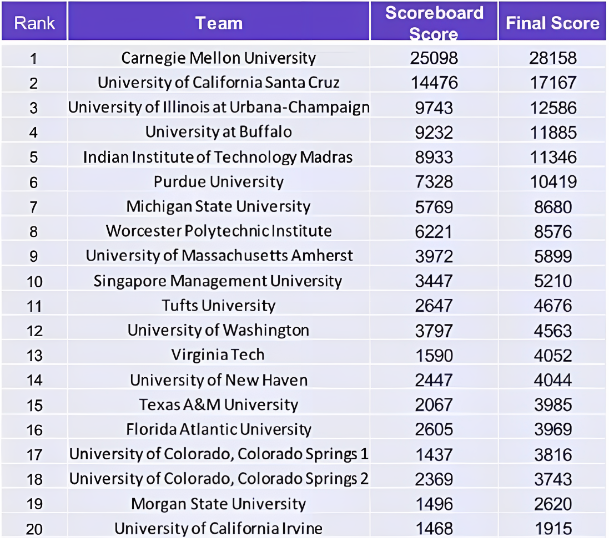
\includegraphics[width=\textwidth]{MITREectf2023.png}         
         \caption{4th in MITRE eCTF'23}
         \label{fig:rank}
     \end{subfigure}
     \begin{subfigure}[b]{0.185\textwidth}
         \centering
         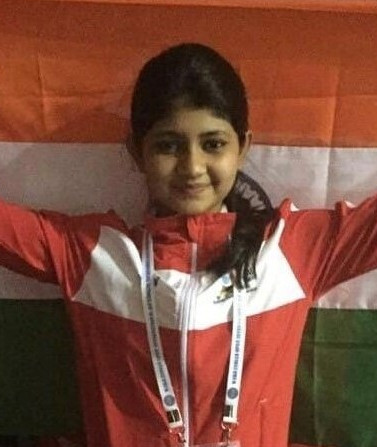
\includegraphics[width=\textwidth]{puhabi.jpg} 
         \caption{Puhabi}
         \label{fig:puhabi}
     \end{subfigure}     
     %\hfill
     \begin{subfigure}[b]{0.44\textwidth}
         \centering
         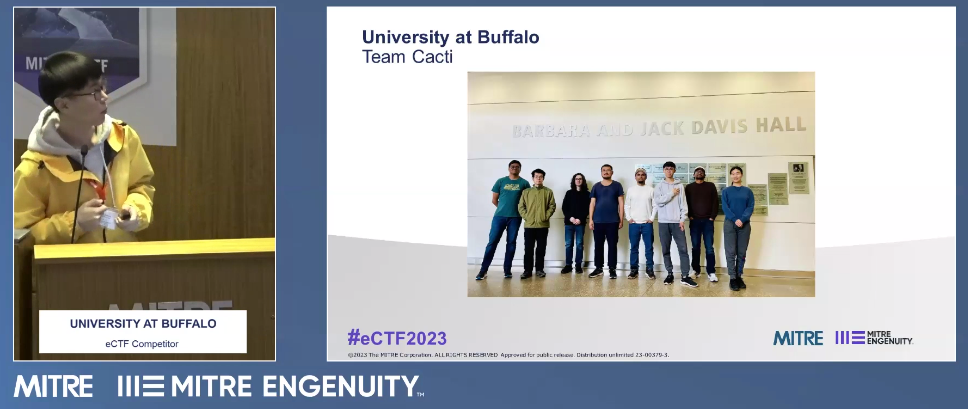
\includegraphics[width=\textwidth]{ectf.png}
         \caption{Team Cacti in eCTF'23 presentation}
         % (Zheyuan Ma, Gaoxiang Liu, Xi Tan, Md Armanuzzaman, Trevor Schupbach, Sagar Mohan, and Hiu Laam Chau)
         \label{fig:presentation}
     \end{subfigure}
     \vspace{-.35cm}      
        \caption{CTF Team and High School Advisee}
        \label{f:ectf}
        \vspace{-.35cm} 
\end{wrapfigure}
\textbf{Cybersecurity Training and CTF Teams with Underrepresented, Undergraduate, and High School Students.}
%The PI will continue to provide students with a safe infrastructure to perform cybersecurity research and develop MCU exploitation and defense skills.
Lead PI Zhao has founded the \emph{Cacti} hacking team with 300+ registered undergraduate and graduate students %(University at Buffalo and Rochester Institute of Technology) 
and over five high school students (Williamsville East high school, Buffalo; Brighton high school, Rochester; and Agartala high school, India).
%Most of registered students are undergraduates from Computer Science, Computer Engineering and Electrical Engineering departments.
%Team \emph{Cacti} competes in embedded and software CTFs. 
Team \emph{Cacti} placed 3rd in the MITRE embedded CTF (eCTF) 2019, 6th in 2020, 9th in 2021, 5th in 2022, 4th in 2023 (as shown in Figure~\ref{fig:rank} and Figure~\ref{fig:presentation}), and 4th in 2024.
%I will also recruit high school students from the Buffalo and Rochester metropolitan areas through the NSF-funded GenCyber Camps.
As shown in Figure~\ref{fig:puhabi}, PI Zhao's high school advisee Puhabi Chakraborti~(female) was conferred the Pradhan award by the Prime Minister Modi of India in 2022~\cite{puhabi2022} and received full scholarship to attend University at Buffalo in 2024.
\ul{Evaluation Plan:} 
The cybersecurity training impacts will be evaluated by student engagement, the number of CTFs team \emph{Cacti} participates, and the team's standings in the CTFs. 
The research experience with underrepresented, undergraduate, and high school students will be evaluated by publications.


\section{Proposed Project Timeline}

\begin{wrapfigure}{r}{0.4\textwidth}
	\vspace{-1cm}
	\definecolor{barblue}{RGB}{153,204,254}
	\definecolor{groupblue}{RGB}{51,102,254}
	\definecolor{linkred}{RGB}{165,0,33}
	\centering
	\begin{ganttchart}%
		[canvas/.style={fill=none, draw=black!84, line width=.35pt},
		hgrid style/.style={draw=black!84, line width=.75pt},
		vgrid={{*3{draw=black!32, line width=.75pt},*1{draw=black!84, line width=.75pt}}},
		title/.style={draw=none, fill=none},
		title label font=\footnotesize,
		title label anchor/.style={below=-1.5ex},
		include title in canvas=false,
		bar label font=\footnotesize\color{black!84},
		bar label anchor/.style={left=0cm},
		bar height=0.3,
		bar/.style={draw=none, fill=black!63},
		bar incomplete/.style={fill=barblue},
		milestone progress label font=\footnotesize\color{black!70},
		group incomplete/.style={fill=groupblue},
		group left shift=0,
		group right shift=0,
		group height=.3,
		group label font=\bfseries\footnotesize,
		group label anchor/.style={left=0cm},
		link/.style={-latex, line width=1.pt, linkred},
		link label font=\footnotesize\bfseries\color{linkred}\MakeUppercase,
		link label anchor/.style={below left=-1.0ex and 0},
		x unit=0.42cm, y unit title=.35cm, y unit chart=0.3cm
		]{1}{12}
		\gantttitle{Year 1}{4}
		\gantttitle{Year 2}{4}
		\gantttitle{Year 3}{4}\\
		\ganttgroup[]%
		{\textbf{Thrust 1}}{1}{5} \\
		\ganttbar[]{Task 1.1}{1}{3} \\
		\ganttbar[]{Task 1.2}{3}{5} \\
		[grid]
		\ganttgroup[]%
		{\textbf{Thrust 2}}{5}{9} \\
		\ganttbar[]{Task 2.1}{5}{6} \\
		\ganttbar[]{Task 2.2}{6}{8} \\
		\ganttbar[]{Task 2.3}{7}{9}\\
		[grid]
		\ganttgroup[]%
		{\textbf{Thrust 3}}{9}{12} \\
		\ganttbar[]{Task 3.1}{9}{10} \\
		\ganttbar[]{Task 3.2}{10}{11} \\
		\ganttbar[]{Task 3.3}{11}{12}
	\end{ganttchart}
	\vspace{-0.4cm}
	\caption{Proposed project timeline}
	\label{fig:timeline}
	\vspace{-2pt}
\end{wrapfigure}
Figure~\ref{fig:timeline} provides a Gantt chart for the tasks outlined in this proposal.
% TODO(glitching): describe the timeline narrative (thrust overlap, CTF, mentoring, etc.)

\section{Results from Prior NSF Support}

% TODO(glitching): update each entry (award #, amount, period, IM/BI, one outcome with citation).
% Each PI must report prior support (or state they have none). In a separate collaborative
% submission, each institution's PI reports their own prior support in their own proposal.
PI Zhao (NEU): \emph{``CAREER: SaTC: Rethinking Trusted Execution Environments for Embedded and IoT Systems"} (CNS-2237238, \$564,748, 2/2023 - 1/2028).
\ul{Intellectual Merit:} Studying a systematic research approach to increase the trustworthiness and deployability of TEEs for embedded and IoT devices.
\ul{Broader Impacts:} Broader significance, beyond securing the IoT infrastructure, includes training the next generation of cybersecurity researchers, educators, and practitioners with deep theoretical understandings and practical skills.
\ul{Research Outcome:} Return-to-non-secure attacks on ARM Cortex-M TrustZone~\cite{ma2023dac}.

PI Tan (UCCS): has not received prior NSF support.

\newpage
\bibliographystyle{ieeetr}
\bibliography{bib, MyPub}
\end{document}
